\subsection{研究方案和技术路线}

\begin{figure}[h]
    \begin{small}
        \begin{center}
            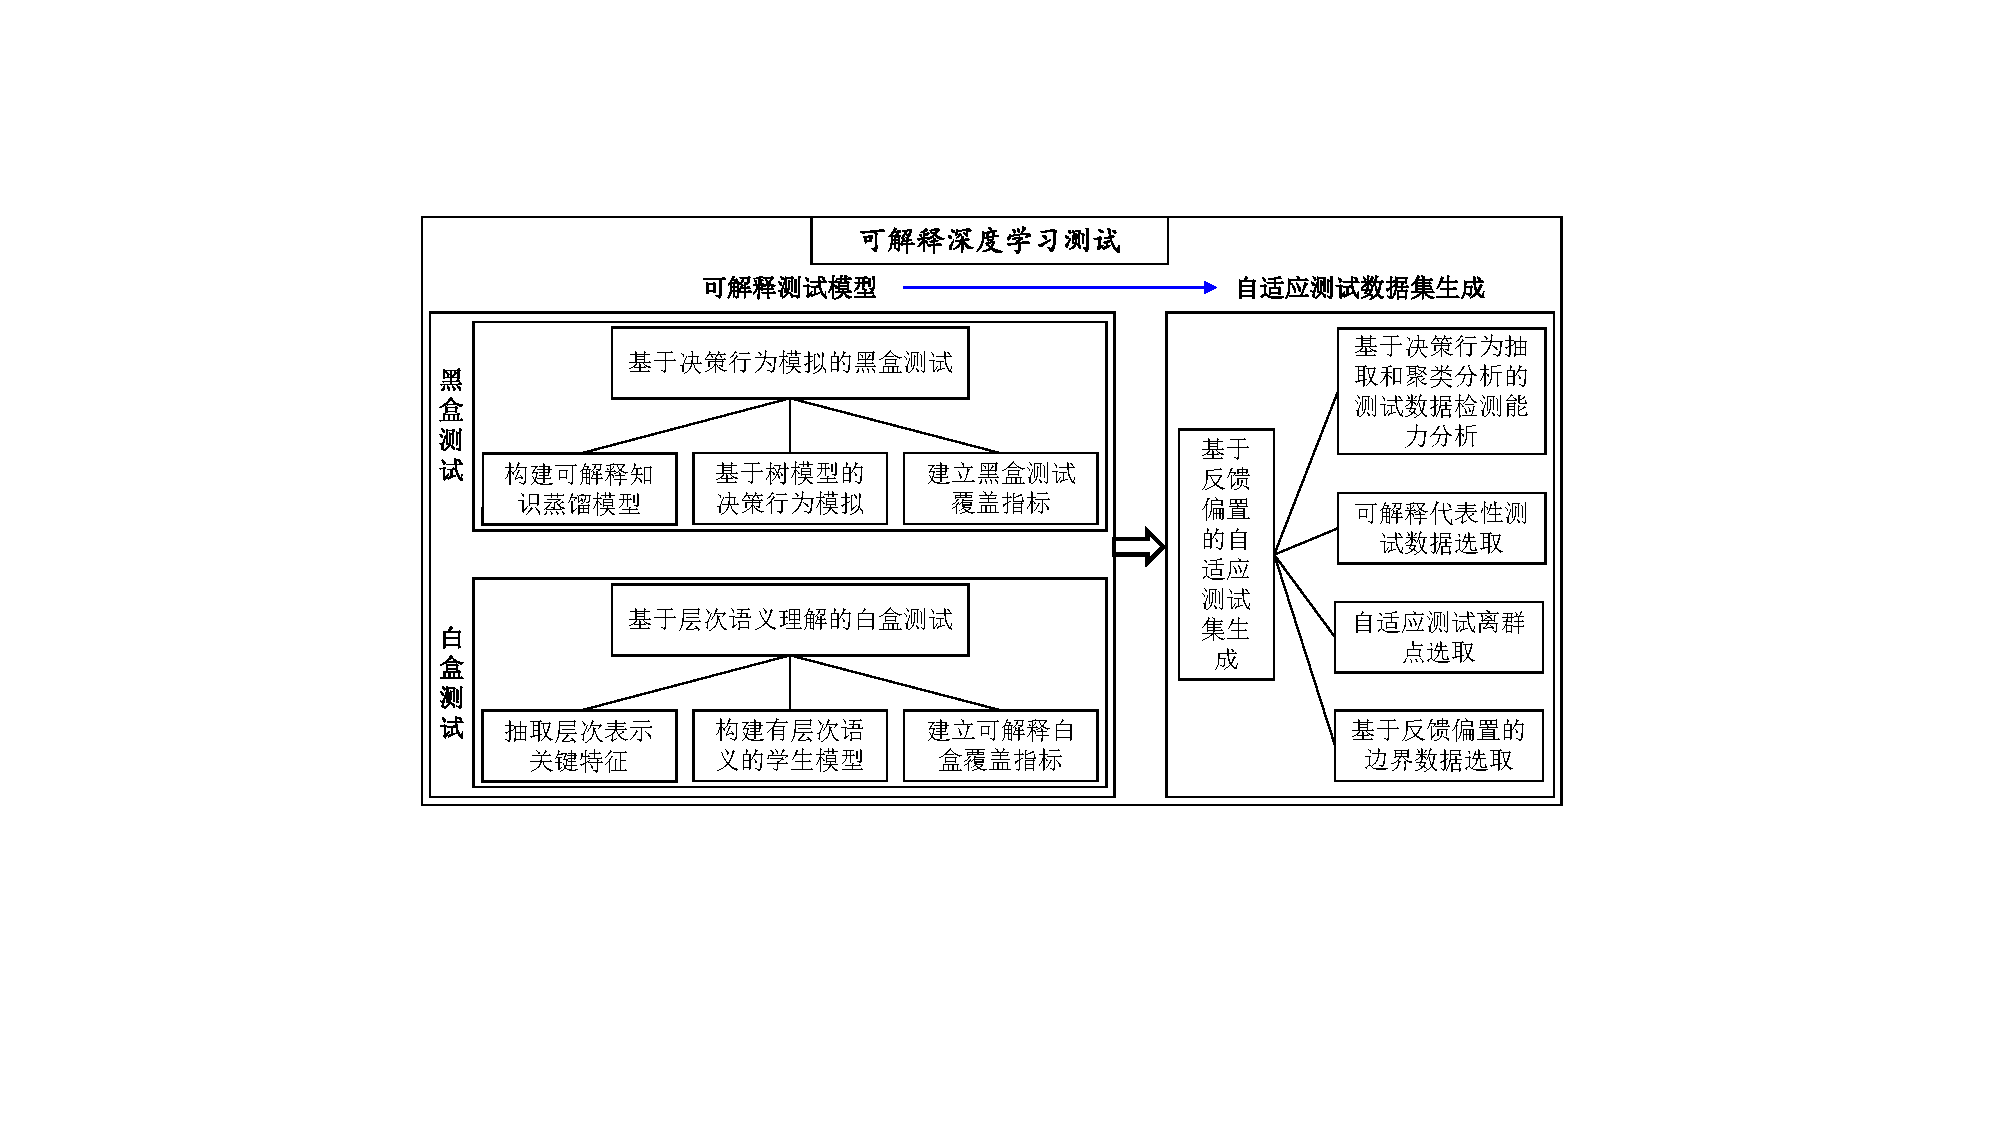
\includegraphics[width=0.95\textwidth]{ch3solution.pdf}
        \end{center}
        \caption{总体技术路线}
        \label{fig:ch3:solution}
    \end{small}
\end{figure}

围绕\ref{ch2content}规划的研究内容和\ref{ch2target}制定的研究目标,本项目拟定的
总体技术路线如\cref{fig:ch3:solution}所示。本项目针对电子医疗记录分析构建基于深
度学习的端到端的解决方案,通过对电子医疗记录数据集依次进行队列识别、EMR插补和可
解释预测,实现对特定患者队列的分析挖掘。本项目的主要研究内容分别对应大数据分析通
用流程中的数据获取、数据预处理和数据分析。此外,鉴于医疗领域的特殊性,本项目的研
究工作需要与医生进行充分的沟通,在模型设计和结果解释等方面融入医生的反馈。下面针
对各部分研究内容,详细介绍其具体研究方案和技术路线。



\subsubsection{基于决策行为模拟的黑盒测试}\label{ch3_1}

\cref{fig:ch3:2Btest}展示了本项目基于决策行为模拟的黑盒测试研究方法,如图所示,
\textbf{本项目拟利用知识蒸馏技术萃取黑盒模型中的知识}。就申请人所知,目前尚未有
基于知识蒸馏的深度学习覆盖度测试研究。首先,本项目利用知识蒸馏技术从黑盒模型(``
教师''模型)中萃取知识,训练一个小模型(``学生''模型)模拟其预测行为,在知识蒸馏
中,``教师''模型被视为黑盒模型,正好契合本项目黑盒测试的场景;其次,本项目拟设计
针对小模型的测试方法,间接评估黑盒模型的泛化能力,一方面,蒸馏得到的``学生''模型
复杂度低,可有效解决深度学习模型测试计算开销大的问题,另一方面,``学生''模型的内
部结构可以自定义,测试者也可访问,本项目拟利用基于树的模型(如:决策树、随机森林
等),以提高测试结果的可解释性。

具体地,给定一个黑盒模型$\mathcal M$,本项目将$\mathcal M$视为``教师''模型,假定
对于任意的输入$x^{(i)}$,测试者仅能得到$\mathcal M$对于该输入预测的概率分布,即
$x^{(i)}$属于各类的概率,记为$p^{(i)}$。$(x^{(i)}, p^{(i)})$的对应关系即为模型
$\mathcal M$中蕴含的知识,将作为训练``学生''模型时的软目标。\textbf{本项目拟构建
基于树的模型作为``学生''模型,记为$\mathcal M_t$,以支持可解释模型测试}。根据知
识蒸馏的思想,在训练``学生''模型时,本项目融合软目标$(x^{(i)}, p^{(i)})$和硬目标
$(x^{(i)}, y^{(i)})$构建``学生''模型的训练目标(Loss),使树型模型的输出同时接近
黑盒模型的概率分布$p^{(i)}$和真实标签$y^{(i)}$。值得注意的是,在训练``学生''模型
时,直接使用``教师''模型SoftMax层的输出结果$p^{(i)}$不合适,因为小模型无法直接学
习得到大模型的效果,我们通过在``学生''模型的损失函数中引入知识蒸馏中的
T(Temperature)参数,放大分类错误的误差,缩小正确分类的误差,可有效提高``学生''
模型训练的效果。

\begin{figure}[htp]
    \begin{small}
        \begin{center}
            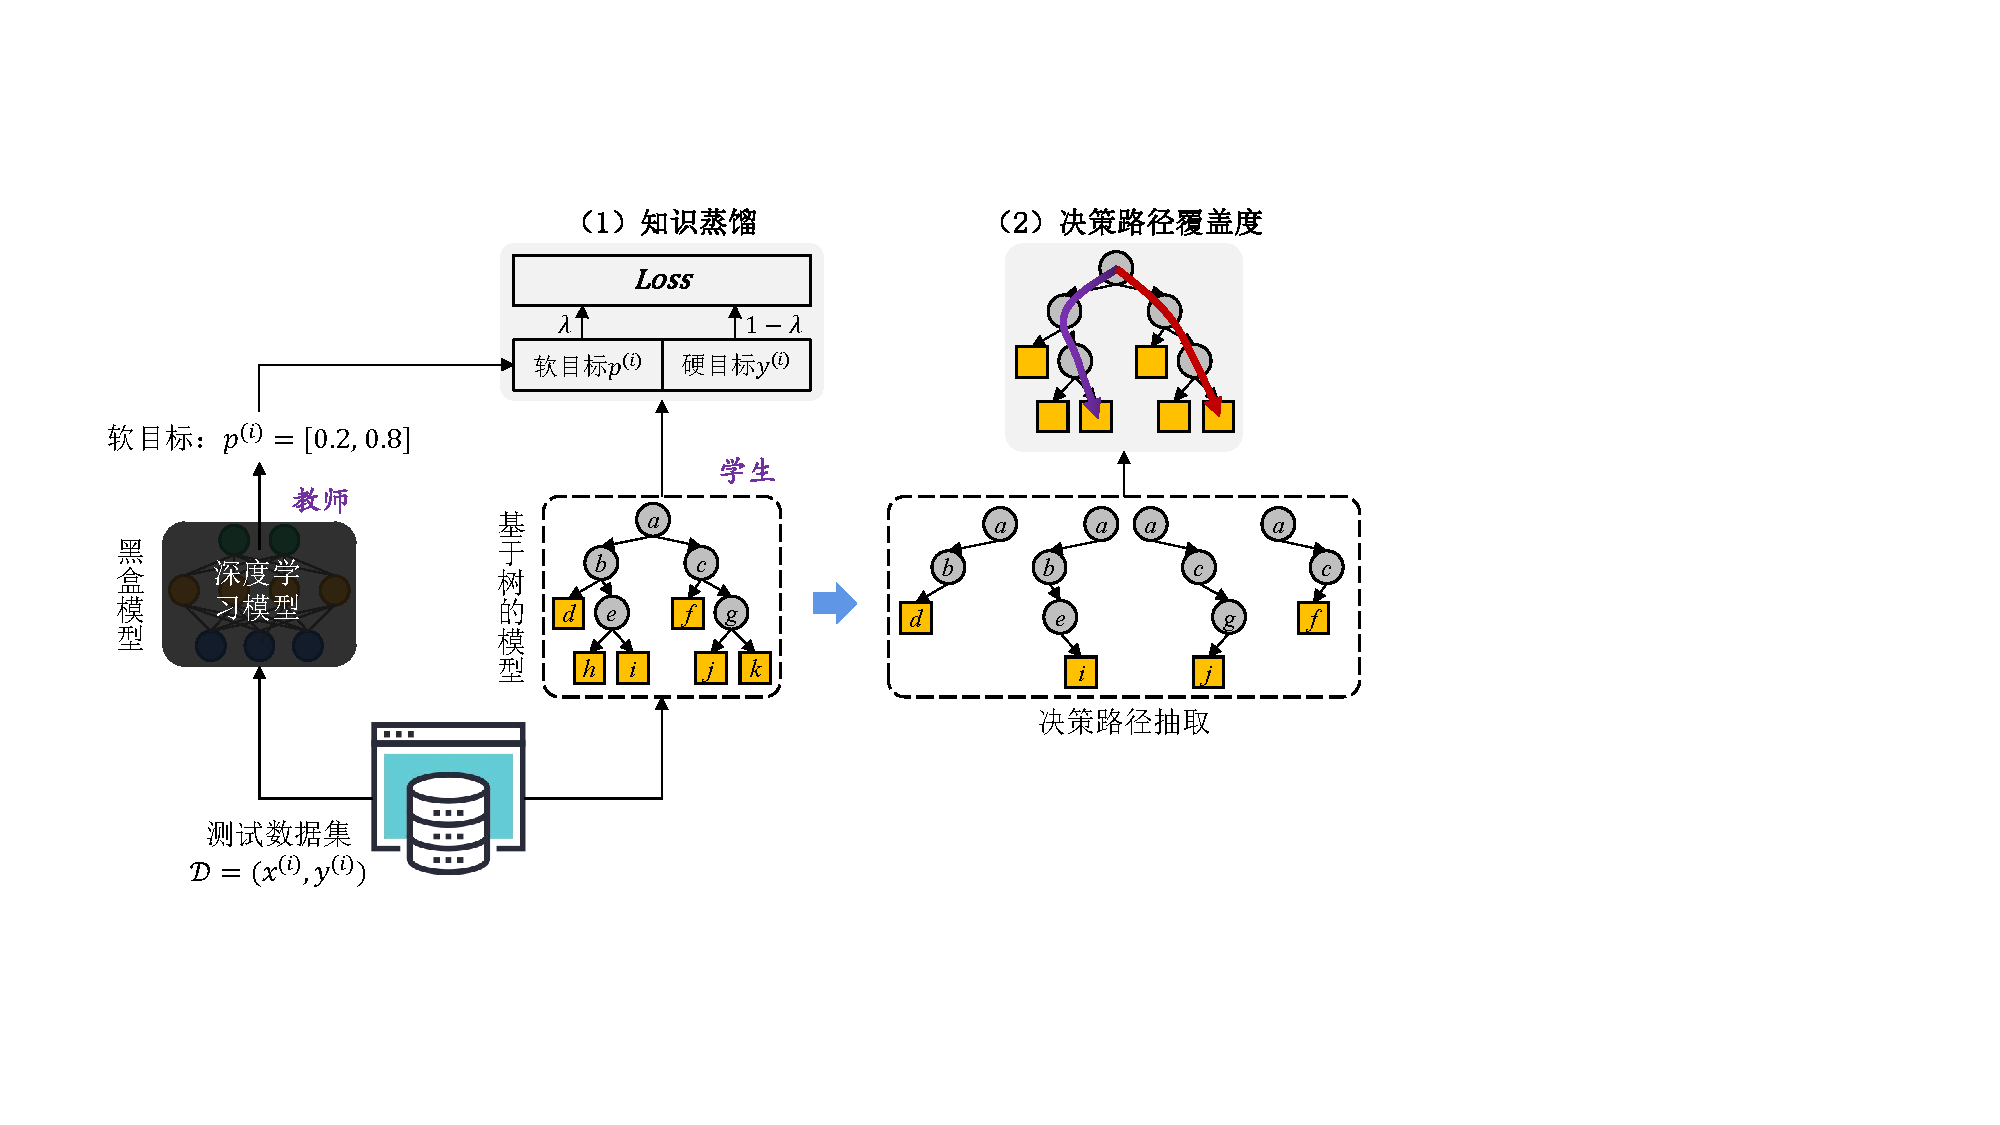
\includegraphics[width=0.9\textwidth]{ch3_2Btest.pdf}
        \end{center}
        \caption{基于决策行为模拟的黑盒测试研究方案}
        \label{fig:ch3:2Btest}
    \end{small}
\end{figure}

\textbf{本项目拟针对``学生''模型建立基于决策路径的覆盖性测试方法},知识蒸馏得到
的``学生''模型$\mathcal M_t$的预测行为非常接近原黑盒模型$\mathcal M$,针对
$\mathcal M_t$的覆盖度测试能比较准确地反映$\mathcal M$的泛化能力。首先,从基于树
的``学生''模型$\mathcal M_t$中抽取该模型对每个测试样本的决策路径,得到路径集合
$\mathcal P=\{t_1, t_2,\dots, t_l\}$,$l$表示路径数。然后,\textbf{本项目拟利用
统计方法建立基于决策路径的覆盖度指标},以评估测试用例集的充分性,其基本思想为对
树模型的决策路径覆盖度高的测试用例集具有良好的充分性,在此基础上,本项目拟计算决
策路径覆盖频率和正态分布的拟合程度来评估测试用例集的分布,可采用
Kolmogorov-Smirnov检验、D检验等方法,并结合正太性检验方法的拟合优度和决策路径的
覆盖度作为测试用例集充分性评价指标。此外,\textbf{本项目拟利用树模型的可解释性,
总结归纳模型错误行为的原因,指导训练数据集扩充和模型优化}。

\subsubsection{融合医学偏差的EMR自动插补}\label{ch3_2}

\begin{comment}
融合医学偏差的EMR自动插补旨在将在时间维度上不规则的电子医疗记录补全为完整的电子
医疗记录,可降低后续预测模型的复杂度和训练时间。电子医疗记录除了反映患者的身体健
康状态,还包含的患者与医院、医生与电子病历系统的交互过程,通常这些附加因素会引入
医学偏差。研究表明,医学偏差可用于对患者更精细的分类,对于理解电子医疗记录有重要
辅助作用,许多医学偏差都会通过医疗特征被记录的时间推断出来,这为建模引入医学偏差
提供了理论基础。本项目利用医疗特征记录的时间和电子医疗记录中缺失值出现的位置,学
习特征的缺失规律,进而将所学缺失规律融入插补模型中。
\end{comment}

\begin{figure}
    \begin{small}
        \begin{center}
            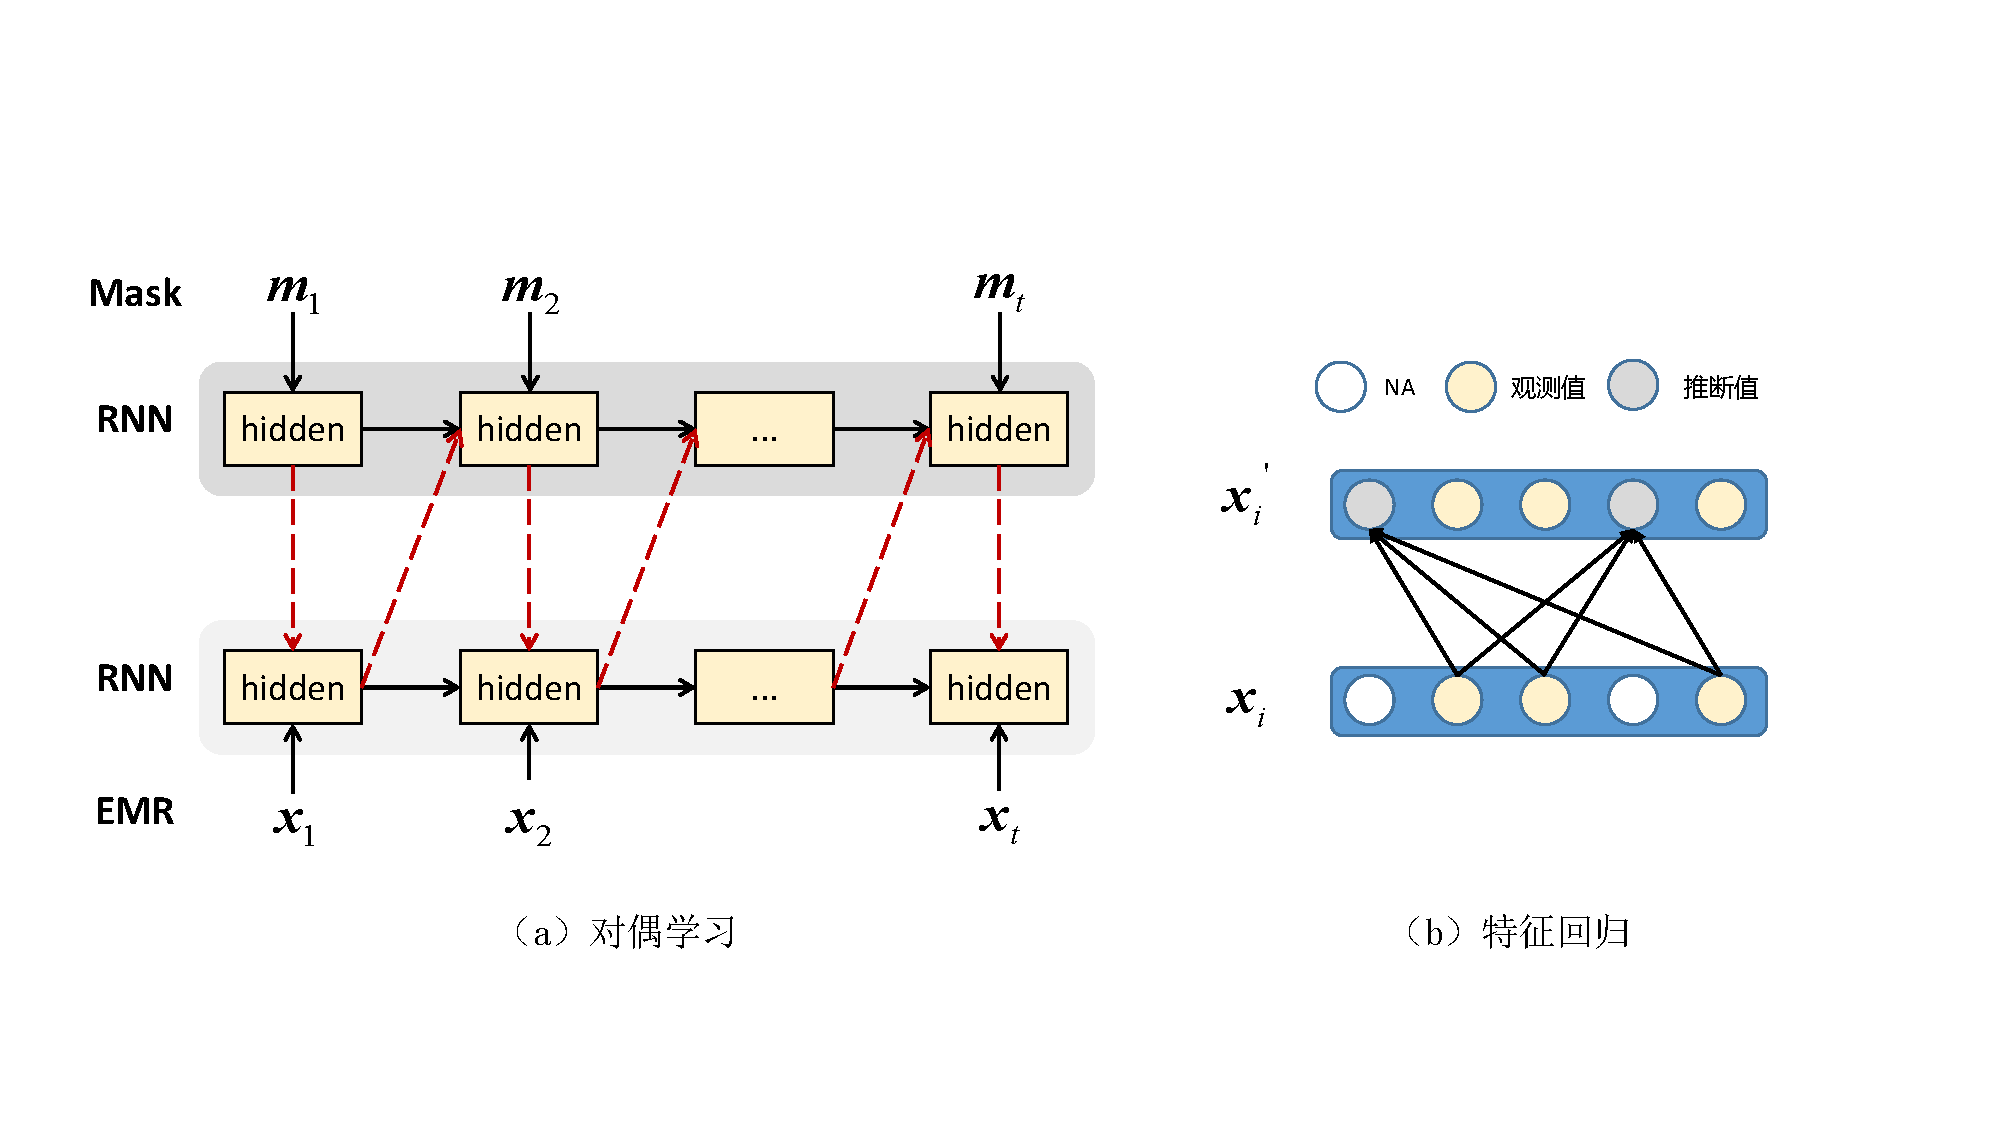
\includegraphics[width=0.95\textwidth]{ch3imputation.pdf}
        \end{center}
        \caption{融合医学偏差的EMR自动插补研究方案}
        \label{fig:ch3:imputation}
    \end{small}
\end{figure}

本项目EMR插补的核心模块如\cref{fig:ch3:imputation}所示。首先,本项目拟针对缺失标
记(即图中的$(\bm m_1, \bm m_2, \dots, \bm m_t)$)建模,如
\cref{fig:ch3:imputation} (a)所示,缺失标记可以反映特征是否被记录,通过对缺失标
记建模,可以得到各个医疗特征在不同时间的缺失规律,即患者医疗特征被记录的规律。同
时,本项目对已经观察到的医疗记录进行建模,这也是缺失值插补最重要的推断基础。我们
发现,在电子医疗记录中,\textbf{缺失矩阵$(\bm m_1, \bm m_2, \dots, \bm m_t)$和观
察到的数据$(\bm x_1, \bm x_2, \dots, \bm x_t)$具有对偶关系},即缺失标记和观测数
据是相互影响的,可作为互相取值推断的参考。以新冠肺炎为例,按照国家卫健委制定的诊
断标准,如果患者2次核酸检测为阴性,则证明其已经康复,所以接下来短时间内患者的核
酸检测结果将会缺失,反之,在医疗条件具备的情况下,如果患者长时间没有被安排核酸检
测,则该患者很可能没有患病,核算检测结果也较大概率为阴性。因此,本项目拟通过对偶
学习方法,融合缺失矩阵和数值矩阵对缺失值进行推测。

其次,电子医疗记录包含多元特征,特征之间一般具有潜在的相互关系,为插补合理的缺失
值,应考虑特征之间的相互关系。如\cref{fig:ch3:imputation} (b)所示,本项目拟在建
模过程中引入\textbf{特征回归}方法,以深度学习模型对特征间关系进行建模,在统一时
间点,若以观察到部分数据,可用它们推断缺失值,这种方法被称为特征回归。
\cref{fig:ch3:imputation} (b)展示的特征回归建模为一个线性层,可以建模为$\bm
x_i^{\prime} = f(\bm W, \bm b; \bm x) = \bm{Wx_i}+\bm b$。

最后,由于不同特征记录时间的差异性,电子医疗记录还具有特征层面的不规则性,即不同
特征的记录时间、记录频率差别很大,所以直接使用原始RNN模型进行EMR插补容易丢失特征
在时间维度方面的信息,因此,本项目拟通过修改GRU(Gated Reccurent Unit)的门机
制,在GRU中引入时间衰减因子,通常而言,特征记录时间离当前时间越远,对患者当前的
状态影响越小,反之,特征记录时间离当前时间越近,则对患者当前的状态影响更大。通过
在GRU中引入时间衰减因子,可以细腻度的控制特征层面的不规则性带来的影响。


\subsubsection{结合特征重要性和时间关联性的可解释预测模型}\label{ch3_3}

电子医疗记录中包含静态特征(如:性别、籍贯等)和动态特征(如:血糖值、慢性肾病分
期等),显然,静态特征随着时间的推移不会发生变化,因此,本项目在构建预测模型时拟
首先针对静态特征和动态特征分别建模,然后将两组特征的向量表示融合起来。

预测模型的可解释性对于临床应用具有重要意义,就电子医疗记录预测性分析而言,模型的
可解释性可以具体化为两方面:1)对于给定研究队列和模型,分析特征的重要性,称为模
型的\textbf{全局可解释性};2)对于某个样本的预测结果,\textbf{提供导致该结果的主
要因素},即一个或者一组具体时间的具体特征值。

由于电子医疗记录中的静态特征远少于动态特征,特征维度较低,本项目拟采取单层全连
接神经网络进行建模,有助于直接计算特征的重要性。对于单个样本预测结果的解释,本项
目拟通过\textbf{深度泰勒分解(Deep Taylor Decomposition)}算法~\citess{montavon2017explaining}分析分析静态特征对预测结果的贡献。对动态特征,本
项目拟采用RNN模型进行建模,虽然RNN能有效捕捉电子医疗记录中的长时间依赖的关系,但
由于其隐含层多次计算,且参数复用,难以通过现有方法得到特征的重要性和具体记录的重
要性。\textbf{本项目拟设计混合注意力机制,解耦时序模型中特征的相互关系和时间的依
赖性}。

\cref{fig:ch3:interpretability}是本项目针对动态特征的可解释性研究方案的示意图,
以图中描述的2个特征为例,首先,为了解耦隐含层是由多个特征计算得到的,我们对输入
$\bm x_i$的每个特征分别计算其隐层表示,然后以拼接的形式组成$\bm x_i$的隐含表示
$\bm h_i = [\bm h_{i1}, \bm h_{i2}]$,这样分开训练虽然避免了特征组合对可解释性的
影响,但这样做会降低模型预测的准确率,本方案利用混合注意力机制实现特征自动组合和
转换,在提高模型可解释性时,也不影响预测性能。

\begin{figure}
    \begin{small}
        \begin{center}
            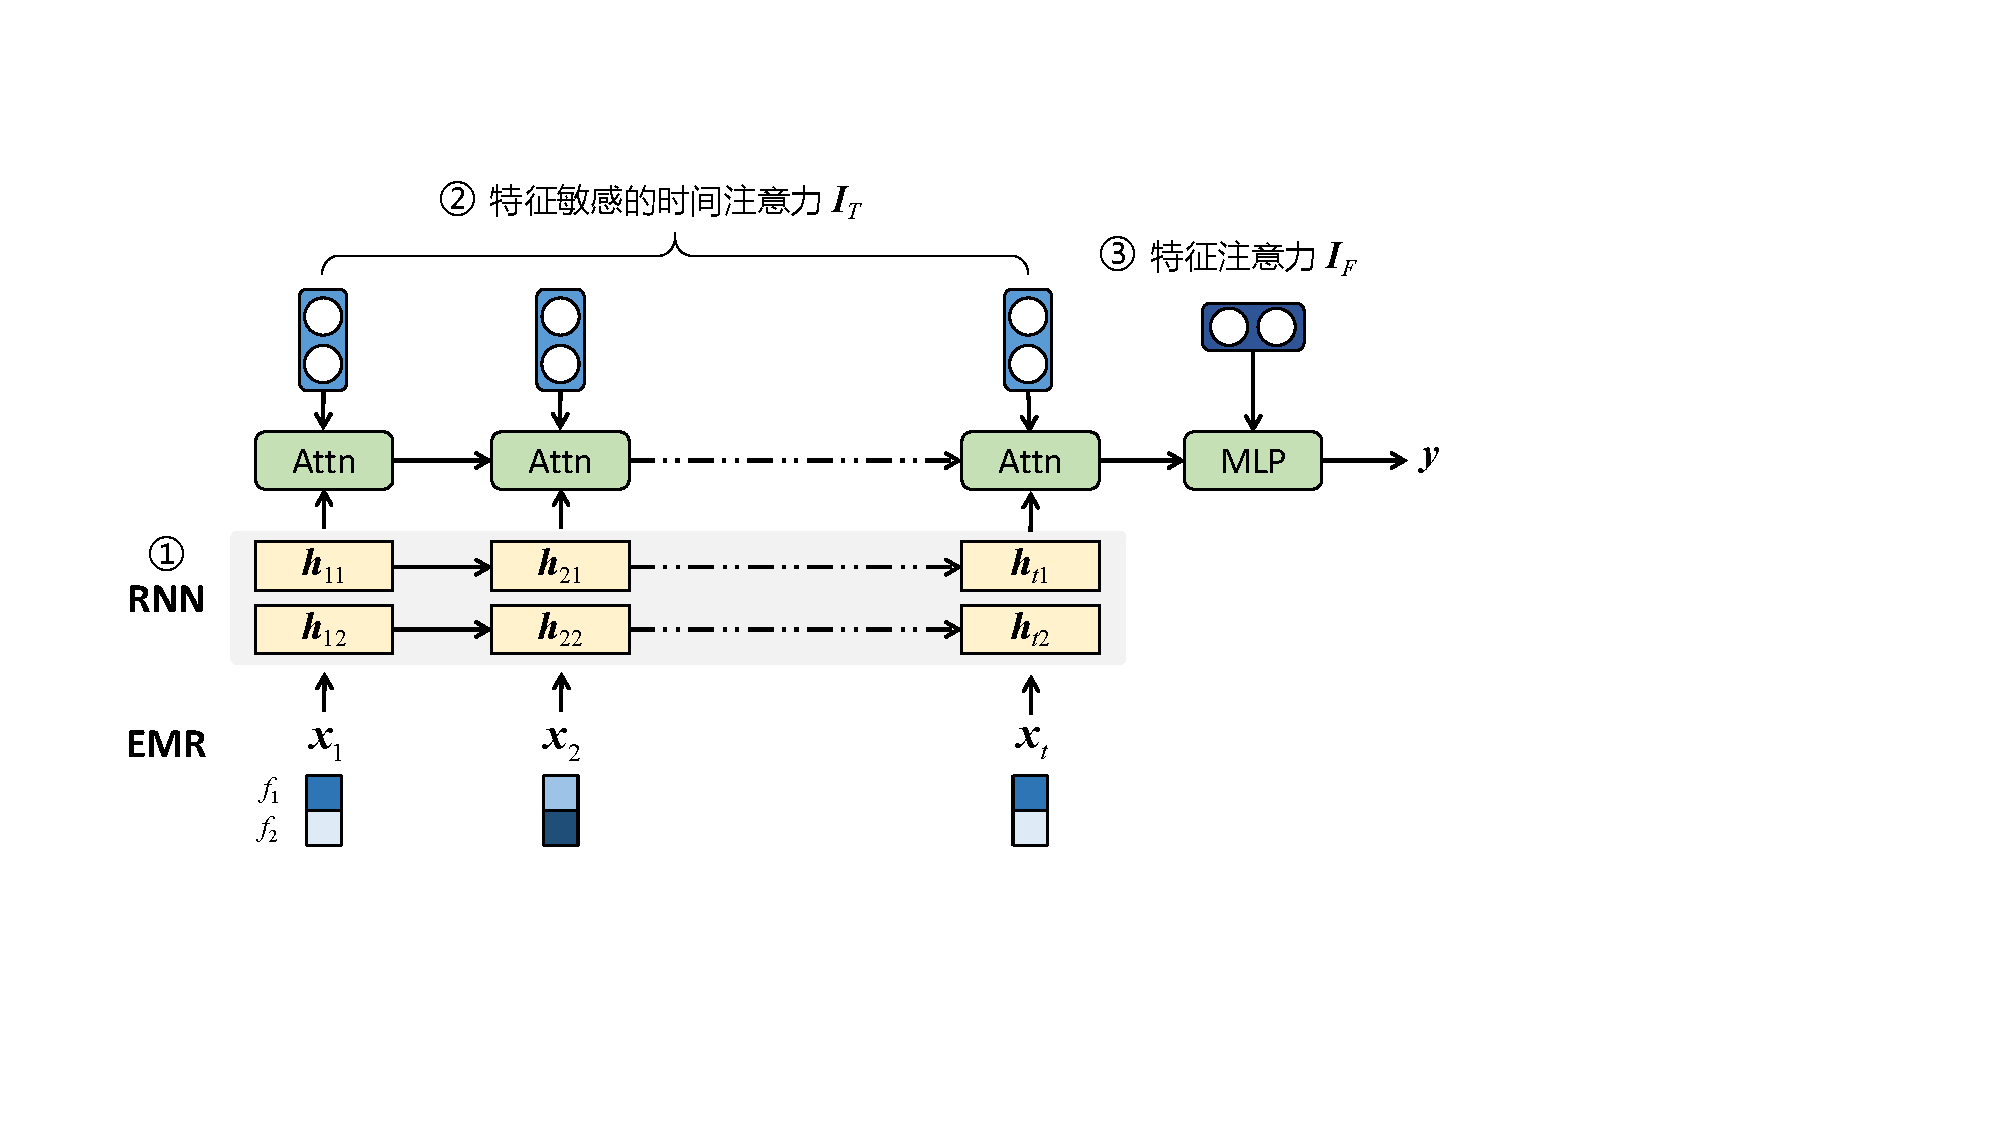
\includegraphics[width=0.85\textwidth]{ch3interpretability.pdf}
        \end{center}
        \caption{可解释预测模型(动态特征)研究方案}
        \label{fig:ch3:interpretability}
    \end{small}
\end{figure}

\textbf{本方案的混合注意力机制包括特征敏感的时间注意力和特征注意力两部分,特征敏
感的时间注意力参数为$\bm I_T \in \mathbb R^{v \times t}$,其中$v$表示特征的个
数,$t$代表时间点的个数}。输入$\bm x_i$的隐含层表示$\bm h_i$通过图中所示的时间注
意力模块(Attn)进行特征融合,具体而言,时间注意的模块的输出为$\bm I_{T_i} \odot
\bm h_i$,其中$\odot$表示沿着时间维度利用特征隐向量乘以注意力权重,即$\bm
I_{T_i} \odot \bm h_i= \sum_{j=1}^v I_{T_{ij}} \bm h_{ij}$。通过引入特征敏感的时
间注意力权重,可学习每个特征在不同时间点(即每条记录)的重要性,而特征注意力参数
$\bm I_F \in \mathbb R^{v}$则用于学习特征的对于模型和预测结果整体重要性,在最后
的全连接层之前与静态特征表示融合并引入模型,以便实现静态特征和动态特征的统一比
较。在此框架下,动态特征的可解释性可建模为以下形式:

\begin{equation}
    \begin{aligned}
        p(\bm y | \bm X) =& \sum_{i=1}^v p(y|z=i, \bm X) P(z=i | \bm X) \\
            =& \sum_{i=1}^v p(y|z=i, I_{T_{1i}} \cdot \bm h_{1i}, I_{T_{2i}} \cdot \bm h_{2i}, \dots, I_{T_{ti}} \cdot \bm h_{ti}) \\
            & \cdot P(z=i|I_{F_1} \cdot \bm h_{t1}, I_{F_2} \cdot \bm h_{t2} \dots, I_{F_v} \cdot \bm h_{tv})
    \end{aligned}
\end{equation}
其中$\bm X= (\bm x_1, \bm x_2, \dots, \bm x_t)$为模型输入,$z$是隐变量,表示数据
特征的编号,$z \in {1,2,\dots, v}$,用于解释不同特征的重要性和时间关联性。
$I_{T_{1i}} \cdot \bm h_{1i}, I_{T_{2i}} \cdot \bm h_{2i}, \dots, I_{T_{ti}}
\cdot \bm h_{ti}$即为特征$i$时间维度的注意力,而$P(z=i|I_{F_1} \cdot \bm h_{t1},
I_{F_2} \cdot \bm h_{t2}, \dots, I_{F_v} \cdot \bm h_{tv})$则为特征$i$的全局重要
性。

\subsubsection{临床预测性任务}

从DKD慢性肾病和急诊科感染性休克的临床需求出发,利用本项目的研究成果,研发预测分
析系统:

首先,熟悉DKD慢性肾病和急诊科感染性休克的医学背景,与医生合作,标注少量符合表现
型的队列数据,利用第(1)节研发的模型从大规模电子医疗记录中筛选出研究队列;其次,
对获得的研究队列进行预处理,分析记录时间分布的特点,利用第(2)节的研究成果对研究
队列进行缺失值补充,并评估数据插补的效果;以第(3)节的核心方法构建可解释预测模
型,评估其预测准确率,并研发特征重要性和时间关联性的可视化系统,展示模型和预测结
果的可解释性分析效果。研究过程中,医生的反馈可作为本项目队列识别、数据插补和可解释模型研究的重要指导,确保本项目研究成果具有实际应用价值。

\subsection{可行性分析}

\subsubsection{理论可行性}

本项目研究目标明确,研究内容清晰,研究方案和技术路线中所应用的方法和技术手段在业
界都有着成熟清晰的理论基础。申请人和项目组对这些关键技术和理论有着深入的了解和掌
握,近年来在人工智能、医疗数据分析等领域的高水平会议上发表了多篇论文。项目组前期
已经对本项目中提到的研究内容分别进行了详细的调研和分析,并在医疗特征表示学习、时
间序列插补等领域取得了初步成果。因此,从理论上说,本项目是可行的。

\subsubsection{技术可行性}

申请人前期调研了大量基于深度学习的电子医疗记录分析的研究工作(如
\ref{relatedwork}节所述),深度学习模型不仅能挖掘高维特征之间复杂的关系,同时能
有效处理数据中长时间依赖关系,非常适合电子医疗记录分析。利用深度学习技术解决电子
医疗记录预测性分析需要解决三个核心问题,即队列识别、EMR不规则性处理和模型的可解
释性,申请人之前的研究工作一直聚焦于电子医疗记录的分析,在医疗特征表示学习、多元
时序数据插补等方面已取得一定的研究成果,并在攻读博士期间与医生合作,参与过医疗分
析系统的开发,相关研发经验可作为本项目的研究基础。申请人所在项目组多年来一直活跃
在在大数据处理和分析、机器学习等领域,在相关领域有着丰富的研究经验和技术积累。同
时,在研究过程中,申请人与医疗机构建立了合作关系,积累了大量可用于实验的真实数据
集。因此,从技术上说,本项目是可行的。

\subsubsection{团队合理性}

项目组在大数据分析和人工智能领域具有一定的基础,积累了丰富的研究经验,在重要国际
会议上发表了多篇高水平论文,项目在信息系统和数据分析系统开发方面也有丰富的积累,
可为本项目可视化分析系统研发提供保障。项目组梯队完善,队伍具有凝聚力和创造力,项
目组成员每周定期讨论,有着良好的科研氛围,同时对本项目的研究内容具有浓厚的研究兴
趣。申请人与联合培养时的导师新加坡国立大学教授Beng Chin Ooi(黄铭钧)一直保持密
切联系,Ooi教授长期研究大数据管理与分析,是数据库和数据挖掘方面非常活跃的科学
家,可为本项目提供技术指导。

申请人与医疗机构和专家一直保持良好的合作关系,与北京大学医疗健康大数据国家研究院
张路霞教授合作研究慢性肾病患者病情进展,和天津市肿瘤医院合作研究肺癌患者治疗效果
评估,同时,申请人参与建设“南开大学-基准联合医学研究中心”,和广州基准医疗有限公
司合作研究基于多模态医疗数据的癌症早诊技术。这些合作单位和专家可为本项目提供专业
意见的反馈,保证研究内容符合医学常识和临床需求。综上所述,项目团队组成合理,能保
障本项目的顺利完成。